\chapter{Quantum Monte Carlo Methods} \label{chp:methods}
%\epigraph{Great quote.}{Author}
\begin{figure}[H]
	\centering
	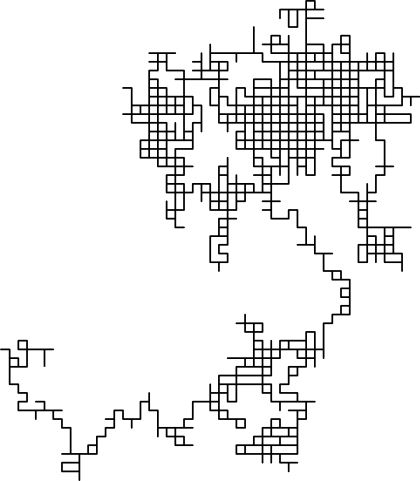
\includegraphics[scale=0.4]{Images/random_walk.png}
	\caption{Random walk on a two-dimensional grid.\\ © Copyright wikipedia.org.}
\end{figure}

Quantum Monte Carlo methods (QMC) is a bunch of \textit{ab initio} methods that attempt to solve the Schrödinger equation using stochastic Monte Carlo integration. \textit{Ab initio} reads "from first principles", which implies that the methods constitute a fundamental approach to the problem. They all seek to evaluate the multi-dimensional integral arising from the Schrödinger equation,
\begin{equation}
E_0= \mel{\Psi_0}{\hat{\mathcal{H}}}{\Psi_0}= \frac{\int d\bs{r}\Psi_0(\bs{r})^*\hat{\mathcal{H}}\Psi_0(\bs{r})}{\int d\bs{r}\Psi_0(\bs{r})^*\Psi_0(\bs{r})},
\label{eq:schrodingergroundstate}
\end{equation}
which provides the ground state energy expectation value for the exact ground state wave function $\Psi_0$. As aforementioned, this integral is analytically infeasible for more or less all systems of interest, rising the need of numerical methods like QMC.

In Monte Carlo integration, we use random numbers to evaluate integrals numerically. Typically, we want to estimate an expectation value $\langle\mathcal{O}\rangle$ by approximating the definition integral with a dense sum,
\begin{equation}
\langle \mathcal{O}\rangle\equiv\int_{-\infty}^{\infty}d\bs{r}P(\bs{r})\hat{\mathcal{O}}(\bs{r})\approx\frac{1}{M}\sum_{i=1}^M\hat{\mathcal{O}}(\bs{r}_i)
\label{eq:montecarlointegration}
\end{equation}
where $M$ is the number of \textit{Monte Carlo cycles} and the coordinates $\bs{r}_i$ are drawn randomly from the probability density function $P(\bs{r})$.

A great advantage of the QMC methods, is that we obtain approximative ground state wave functions when solving equation \eqref{eq:schrodingergroundstate}, which by the fourth postulate of quantum mechanics let us estimate ground state expectation values associated with other operators as well. 

Two widely popular QMC methods are the variational Monte Carlo method (VMC) and the diffusion Monte Carlo method (DMC), where the former is arguably the simplest of all the QMC methods. It attempts to directly solve the integrals in equation \eqref{eq:schrodingergroundstate} by varying parameters, with the support of the variational principle presented in section \ref{sec:variationalprinciple}. This makes VMC a comparably computationally cheap method, but the performance is not in the league of the best methods.

DMC, on the other hand, is computationally expensive, but is also potentially numerically exact, making it a preferred method when high accuracy is needed. At first glance it might seems like a tradeoff where VMC is used when computational time is more important than the accuracy and DMC is used when the opposite is true. However, DMC requires a wave function input which is close to the exact wave function, forcing us to first run VMC to obtain this wave function before the DMC machinery can be started.

As VMC is our main focus in this work, it will be explained thoroughly in this chapter together with common sampling techniques. In the end we will briefly explain the idea behind the DMC method, but since this method is not implemented it will not be our main priority.

\section{Variational Monte Carlo} \label{subsec:vmc}
The variational Monte Carlo method (hereafter VMC) is today widely used when it comes to the study of ground state properties of quantum many-body systems. It makes use of Markov chain Monte Carlo methods, often abbreviated MCMC, where the particles are assumed to be moving in Markov chains controlled by Monte Carlo simulations. Going back to the variational principle in equation \eqref{eq:variationalprinciple}, one observes that by choosing an approved wave function, one gets an energy larger or equal to the ground state energy. \bigskip

Before we present the mathematical framework of the method, we will restate the two big problems in many-body physics, mentioned in the introduction:
\begin{enumerate}
	\item The many-body energy expectation value is analytically infeasible for most systems
	\item The correct many-body wave function is generally unavailable
\end{enumerate}

\subsection{Approaching the first problem}
Let us first address the first problem, which often is considered as the root of all evil in many-body physics. In chapter \ref{chp:quantum}, we saw that the two-body interaction term makes the integral impossible to solve for many particles, such that we need to rely on numerical methods. 

In VMC, we start with a trial wave function guess $\Psi_T(\bs{r};\bs{\theta})$ where the parameters $\bs{\theta}$ are varied to minimize the energy. According to the variational principle, the obtained energy will always be higher or equal to the true ground state energy, where the equality is the case if and only if the wave function is the exact ground state wave function. Denoting the exact ground state energy by $E_0$ and the obtained energy as $E$, we can summarize this by
\begin{equation}
E_0 \leq E = \frac{\int d\bs{r}\Psi_T(\bs{r})^*\hat{\mathcal{H}}\Psi_T(\bs{r})}{\int d\bs{r}\Psi_T(\bs{r})^*\Psi_T(\bs{r})}.
\end{equation}
Furthermore, the integral can be written on the form of a general expectation value
\begin{equation}
E = \int d\bs{r} E_L(\bs{r})P(\bs{r})
\end{equation}
defining the local energy as
\begin{equation}
E_L(\bs{r})\equiv\frac{1}{\Psi_T(\bs{r})}\hat{\mathcal{H}}\Psi_T(\bs{r})
\label{eq:localenergy}.
\end{equation}
$P(\bs{r})$ is called the probability density function (PDF), was first introduced in equation \eqref{eq:pdf} and in a more general scheme the PDF reads
\begin{equation}
P(\bs{r})=\frac{|\Psi_T(\bs{r})|^2}{\int d\bs{r}|\Psi_T(\bs{r})|^2}.
\label{eq:probvmc}
\end{equation}
Since the energy expectation value now is on the form of a general expectation value, we can use the approximation set up by Monte Carlo integration in equation \eqref{eq:montecarlointegration}, yielding 
\begin{equation}
E \approx \frac{1}{M}\sum_{i=1}^ME_L(\bs{r}_i) \label{eq:energysum}.
\end{equation}
We recall that the local energies $E_L(\bs{r}_i)$ are evaluated with particle configurations $\bs{r}_i$ drawn from $P(\bs{r})$. In this manner the obtained energy is guaranteed to approach the exact energy as the number of Monte Carlo cycles, $M$, increases. Actually, the standard error goes as $\mathcal{O}(1/\sqrt{M})$, making the method pretty accurate for large numbers of cycles. In the limit $M\rightarrow\infty$, the error goes to zero,
\begin{equation}
\langle E_L\rangle=\lim_{M\to\infty} \frac{1}{M}\sum_{i=1}^ME_L(\bs{r}_i),
\end{equation}
indicating the desire of largest number of cycles. This is associated with a zero-variance property governing the VMC method, stating that the variance in the true ground state should be zero. For more statistical details, see \cite{deb_variational_2014}. Various sampling regimes are described in section \ref{sec:metropolis}.

\subsection{Approaching the second problem}
So far so good, but how do we attack the second problem stated above? One of the big strengths of VMC, as aforesaid, is that we obtain an approximative wave function meanwhile the energy expectation value is estimated. If we go back to equation \eqref{eq:localenergy}, we see that a PDF is required in order to estimate the energy, which again is based on a wave function. 

In VMC, we need to "guess" an initial trial wave function, $\Psi_T(\bs{r},\bs{\theta})$, which hopefully is close to the exact wave function. The parameters, $\theta$, are then updated in order to minimize $\langle E_L\rangle$, such that the energy gets lower for each \textit{iteration}. If the estimated energy approaches the ground state energy, we also assume that the wave function approaches the ground state wave function. Consequently, we will end up with a more or less accurate wave function approximation when the energy has converged. 

As a notice, the term \textit{iterations} should not be confused with the term \textit{cycles}. For each iteration, we run $M$ Monte Carlo cycles and then update the parameters. The parameter update is discussed in section \ref{sec:parameterupdate}.

\subsection{Common extensions}
This finalizes the essential theory behind the VMC method. However, a sampling algorithm is needed to draw samples randomly from $P(\bs{r})$, and in section \ref{sec:metropolis} some popular sampling techniques are described. Before we jump into this field, we will discuss some usual extensions and improvements to the VMC method.

Initially, the particle configuration $\bs{r}$ might not be representative for a configuration in equilibrium, making the first cycles a poor estimate of the expectation value. An easy fix to this problem is to basically ignore the first sampling period, known as the \textit{burn-in period}. With this in mind, we implement an equilibriation fraction describing the fraction of the total number of cycles that is used in the burn-in period. When running multiple parallel processes, the burn-in period should be the same for all the processes.

We also have a technique called \textit{thinning}, which means picking every $n$'th sample in the chain and ignore the rest. This is shown to give a more or less identical expectation value and makes the program less memory-requiring, but due to worse statistics, this should be avoided as long as there is no lack of memory. 

\section{The Metropolis algorithm} \label{sec:metropolis}
Metropolis sampling is a Markov chain Monte Carlo method, which generates a Markov chain using a proposal density for new steps, and the method also rejects unsatisfying moves. In its most simple form, a particle is moved in a random direction, which was the original method invented by Metropolis et.al. back in 1953 \cite{metropolis_equation_1953}. Later, the method was improved by Hastings et.al., giving rise to the more general Metropolis-Hastings algorithm \cite{hastings_monte_1970}.
The genius of the Metropolis algorithms, is that the acceptance of a move is not based on the probabilities themselves, but the ratio between the new and the old probabilities. In that way, we avoid calculating normalizing factor, which is often computational intractable.

We will first discuss Markov chains in general, before we connect them to the original Metropolis algorithm, henceforth called \textit{brute-force sampling}, and then the Metropolis-Hastings algorithm, also called \textit{importance sampling}.

If we denote $\bs{r}$ as the current state, and $\bs{r}'$ as the proposed state, we have a transition rule $P(\bs{r}'|\bs{r})$ for going from $\bs{r}$ to $\bs{r}'$ and a transition rule $P(\bs{r}|\bs{r}')$ for going the opposite way. If we then assume that the rules satisfy \textit{ergodicity} and \textit{detailed balance}, we have the following relationship:
\begin{equation}
P(\bs{r}'|\bs{r})P(\bs{r})=P(\bs{r}|\bs{r}')P(\bs{r}'),
\end{equation}
which is actually a restatement of Bayes' theorem presented in section \ref{sec:bayes}.

The next step is to rewrite the transition rules in terms of a proposal distribution $T(\bs{r}'|\bs{r})$ and an acceptance probability $A(\bs{r}',\bs{r})$,
\begin{equation}
P(\bs{r}'|\bs{r})=T(\bs{r}'|\bs{r})A(\bs{r}',\bs{r}).
\end{equation}
In order to satisfy the detailed balance, we need to choose $A(\bs{r}',\bs{r})$ such that
\begin{equation}
A(\bs{r}',\bs{r})=\text{min }\left[1,\frac{T(\bs{r}|\bs{r}')P(\bs{r}')}{T(\bs{r}'|\bs{r})P(\bs{r})}\right],
\label{eq:acceptance}
\end{equation}
since $A$ cannot be larger than 1. We want to accept a move with probability $A(\bs{r}',\bs{r})$. One way to do that is to draw a number from a uniform distribution between 0 and 1. If this number is lower than the acceptance, the move should be accepted. Otherwise it will be rejected.

\subsection{Brute-force sampling} \label{sec:bruteforce}
In its simplest form, the move is proposed randomly both in magnitude and direction. Mathematically, we can write this as
\begin{equation}
\bs{r}'=\bs{r}+\Delta xd\bs{r}
\end{equation}
where $\Delta x$ is the step length and $d\bs{r}$ has a random magnitude and direction (typically which particle to move). We obtain the naive acceptance probability when requiring $T(\bs{r}'|\bs{r})=T(\bs{r}|\bs{r}')$, such that the it simplifies to
\begin{equation}
A(\bs{r}',\bs{r})=\text{min }\left[1,\frac{P(\bs{r}')}{P(\bs{r})}\right].
\end{equation}

However, with this approach an unsatisfying number of moves will be rejected, which results in a significant waste of computing power. A better method is \textbf{importance sampling}, since the particles are moved according to the quantum force. 

\subsection{Importance sampling} \label{sec:importancesampling}
Importance sampling is a more intelligent sampling method than the brute-force sampling, since the new position is based on an educated guess. To understand how it works, we need to take a quick look at diffusion processes. We start from the Fokker-Planck equation,
\begin{equation}
\frac{\partial P(\bs{r},t)}{\partial t}=D\nabla\left(\nabla-\bs{F}\right)P(\bs{r},t)
\label{eq:fokkerplanck}
\end{equation}
which describes how a probability distribution $P(\bs{r},t)$ evolves in appearance of a drift force $\bs{F}$. In the case $\bs{F}=0$, the equation reduces to the diffusion equation with $D$ as the diffusion constant. This simplifies to $D=1/2$ in natural units. 

The Langevin equation states that a diffusion particle tends to move parallel to the drift force in the coordinate space, with $\bs{\eta}$ introducing some random noise. The equation reads
\begin{equation}
\frac{\partial \bs{r}(t)}{\partial t}=D\bs{F}(\bs{r}(t))+\bs{\eta}.
\label{eq:langevin}
\end{equation}
Given a position $\bs{r}$, the new position $\bs{r}'$ can be be found by applying forward-Euler on the Langevin equation, obtaining
\begin{equation}
\bs{r}'=\bs{r}+D\Delta t\bs{F}(\bs{r}) + \bs{\xi}\sqrt{\Delta t}
\end{equation}
where $\Delta t$ is a fictive time step and $\bs{\xi}$ is a Gaussian random variable. Further, we want to find an expression of the drift force $\bs{F}$ which makes the system converge to a stationary state. A stationary state is found when the probability density function, $P(\bs{r})$, is constant in time, i.e, when the left-hand-side of Fokker-Planck is zero. In that case, we can rewrite the equation as
\begin{equation}
\nabla^2P(\bs{r})=P(\bs{r})\nabla\bs{F(\bs{r})}+\bs{F(\bs{r})}\nabla P(\bs{r}).
\end{equation}
where the parenthesis are written out and we have moved the term independent of the force $\bs{F}$ to the left-hand-side. Moreover, we assume that the drift force takes the form $\bs{F(\bs{r})}=g(\bs{r})\nabla P(\bs{r})$ based on the fact that the force should point to a higher probability. We can then go ahead and write
\begin{equation}
\nabla^2 P(\bs{r})\big(1-P(\bs{r})g(\bs{r})\big)=\nabla\big(g(\bs{r})P(\bs{r})\big)\nabla P(\bs{r})
\end{equation}
where the quantity $\nabla^2 P(\bs{r})$ is factorized out from two of the terms. The equation is satisfied when $g(\bs{r})=1/P(\bs{r})$, such that the drift force evolves to the well-known form
\begin{equation}
\bs{F}(\bs{r})=\frac{\nabla P(\bs{r})}{P(\bs{r})}=2\frac{\nabla\Psi_T(\bs{r})}{\Psi_T(\bs{r})}=2\nabla\ln\Psi_T(\bs{r}),
\end{equation}
which is also known as the \textit{quantum force}.

The remaining part concerns how to decide if a proposed move should be accepted or not. For this, we need to find the sampling distributions $T(\bs{r}'|\bs{r})$ from equation \eqref{eq:acceptance}, which are just the solutions of the Fokker-Planck equation. The solutions read
\begin{equation}
G(\bs{r}',\bs{r},\Delta t)\propto\exp\Big(-\big(\bs{r}'-\bs{r}-D\Delta t\bs{F}(\bs{r})\big)^2/4D\Delta t\Big)
\end{equation}
which is categorized as a Green's function. In general, the essential property of any Green's function is that it provides a way to describe the response of an arbitrary differential equation solution. For our particular case, it correspond to the normal distribution centered around $\mu=\bs{r}+D\Delta t \bs{F}(\bs{r})$ with variance $\sigma=2D\Delta t$, $\mathcal{N}(\bs{r}'|\bs{r}+D\Delta t \bs{F}(\bs{r}),2D\Delta t)$. By utilizing this, the acceptance probability for the importance sampling can finally be written as
\begin{equation}
A(\bs{r}'|\bs{r})=\text{min }\left[1,\frac{G(\bs{r},\bs{r}',\Delta t)P(\bs{r}')}{G(\bs{r}',\bs{r}, \Delta t)P(\bs{r})}\right],
\end{equation}
where the marginal probabilities are still given by equation \eqref{eq:probvmc}. 

\subsection{Gibbs sampling}
Gibbs sampling has throughout the years gained high popularity in the machine learning community when it comes to training Boltzmann machines. There are probably many factors that contribute to this, where the performance obviously is one of them. Another relevant motivation is the absent of tuning parameters, which makes the method easier to deal with compared to many of its competitors. 

The method is an instance of the Metropolis-Hastings algorithm, and is therefore classified as another Markov chain Monte Carlo method. It differs from the Metropolis methods discussed above by the fact that all the moves are accepted, such that we do not waste computational time on rejected moves. Nevertheless, we should not use this argument alone to motivate the use of Gibbs sampling, as less than 1\% of the moves in importance sampling is usually rejected.

We will in the following briefly describe the mathematical foundation of the method, before we, for the sake of clarity, connect it to the restricted Boltzmann machines. The method is built on the concept that, given a multivariate distribution, it is simpler to sample from a conditional distribution than to marginalize by integrating over a joint distribution. This is the reason why we do not need the marginal distributions in Gibbs sampling, but rather the conditional distributions. In the most general, Gibbs sampling proposes a rule for going from a sample $\bs{x}^{(i)}=(x_1^{(i)},x_2^{(i)},\hdots,x_n^{(i)})$ to another sample $\bs{x}^{(i+1)}=(x_1^{(i+1)},x_2^{(i+1)},\hdots,x_n^{(i+1)})$, similar to the Metropolis algorithm. However, in Gibbs sampling the transition from $x_j^{(i)}$ to $x_j^{(i+1)}$ is performed according to the conditional distribution specified by
\begin{equation}
P\big(x_j^{(i+1)}|x_1^{(i+1)},\hdots,x_{j-1}^{(i+1)},x_{j+1}^{(i)},\hdots,x_n^{(i)}\big).
\end{equation}
The marginal distribution of a subset of variables can then be approximated by simply considering the samples for that subset of variables, ignoring the rest. 

For a restricted Boltzmann machine, this becomes a two-step sampling process due to the latent variables, such that we use the conditional probabilities $P(\bs{r}|\bs{h})$ and $P(\bs{h}|\bs{r})$ to update the visible and hidden units respectively. For the restricted Boltzmann machine with Gaussian-binary units presented in section \ref{sec:RBM}, the conditional probability of $h_j=0$ given a set of visible nodes $\bs{x}$ is
\begin{equation}
P(h_j=0|\bs{x})=\frac{1}{1+\exp(+b_j+\sum_{i=1}^Nx_iw_{ij}/\sigma^2)}
\end{equation}
and the corresponding conditional probability of $h_j=1$ is
\begin{equation}
P(h_j=1|\bs{x})=\frac{1}{1+\exp(-b_j-\sum_{i=1}^Nx_iw_{ij}/\sigma^2)},
\end{equation}
which is by the way the sigmoid function again. Note that $P(h_j=0|\bs{x})+P(h_j=1|\bs{x})=1$, indicating that a hidden node $h_j$ can only take 0 or 1, hence binary. When updating the hidden node, one typically calculate the sigmoid $P(h_j=1|\bs{x})$ and set $h_j$ to 1 if this probability is larger than 1/2, and set it to 0 otherwise. 

For the update of the visible nodes, we see from equation \eqref{eq:normal} that the visible nodes are chosen after the normal distribution,
\begin{equation}
P(x_i|\bs{h})=\mathcal{N}\Big(a_i+\sum_{j=1}^Hw_{ij}h_j,\sigma^2\Big)
\end{equation}
which introduce some stochasticity to the system. By going back and forth in the Boltzmann machine multiple times (a round trip corresponds to an iteration), the hope is that the expectation values can be approximated by averaging over all the iterations. 

As pointed out earlier, the Gibbs sampling will not be implemented in this work, but is described for completeness purposes. The reason for this, is that the method has not shown promising results for our specific problem, and we will instead rely on Metropolis sampling. We have already tested the Gibbs sampling in another similar project on small quantum dots \cite{nordhagen_computational_2018}, and so have others like Vilde Flugsrud \cite{flugsrud_vilde_moe_solving_nodate}. The results are matching and show poor performance compared to the Metropolis-Hastings algorithm.

However, the Gibbs sampling method itself should not be underestimated. Carleo and Troyer showed its importance when solving the Ising model using a restricted Boltzmann machine and Gibbs sampling, and in traditional Boltzmann machines the Gibbs sampling is the preferred tool \cite{carleo_solving_2017}.

\iffalse
\subsection{Similarities between Gibbs and Metropolis sampling}
Based on the previous section, it might be hard to recognize the similarities between Gibbs sampling and the Metropolis sampling methods. However, the connection between them is important for several reasons. Firstly, this can lead us to the link between standard restricted Boltzmann machines and standard VMC, as Boltzmann machines often are based on Gibbs sampling and VMC often is based on the Metropolis samplings. We need to exploit this link to take fully advantage of the Boltzmann machines. Secondly, this might clarify why the Gibbs sampling does not serve our purpose.

In chapter \ref{chp:systems}, we presented the relation between a quantum system and expressions of the Hamiltonian, which is the energy operator. In section \ref{sec:unsupervised}, we described how Boltzmann machines are defined and how one can find the energy of a Boltzmann machine. Further, we looked at the updating schemes, which for both cases corresponds to minimizing the cost function and maximizing the log-likelihood function. 

All in all, there are many similarities between the two methods. They are fundamentally related through Markov random fields, ...
\fi

\section{Parameter update} \label{sec:parameterupdate}
Above we have discussed the sampling in detail, which is a central part of the VMC method. Another important part is obviously the \textit{variation} of the parameters, which is needed in order to finding an approximative wave function. In section \ref{sec:optimizationalgorithms}, we discussed various gradient based optimization algorithms for iterative minimization of the cost function in machine learning, and the same methods can be used in VMC. Given a cost function $\mathcal{C}(\bs{\theta})$, the gradient with respect to a parameter $\theta_j$ can be found from
\begin{equation}
\nabla_{\theta_j} \mathcal{C}(\bs{\theta})\equiv\frac{\partial \mathcal{C}(\bs{\theta})}{\partial \theta_j},
\end{equation}
where we henceforth use the short-hand notation with $\nabla$ representing the gradient. 

However, we need to define a cost function for VMC which is minimized when the ground state energy is obtained. According to the variational principle, the ground state energy is the lowest energy we can obtain, so an obvious cost function is the energy expectation value. We therefore set
\begin{equation}
\mathcal{C}(\bs{\theta})=\langle E_L\rangle
\end{equation}
since we get the expectation value of the local energy from the Metropolis sampling. Further, we use the definition of the gradient of an expectation value and obtain
\begin{equation}
\nabla_{\theta_j} \langle E_L\rangle=2\Big(\langle E_L\nabla_{\theta_j}\ln\Psi_T\rangle - \langle E_L\rangle\langle\nabla_{\theta_j}\ln\Psi_T\rangle\Big)
\label{eq:gradientenergy}
\end{equation}
which means that we need to calculate the expectation values $\langle E_L\nabla_{\theta_j}\ln\Psi_T\rangle$ and $\langle\nabla_{\theta_j}\ln\Psi_T\rangle$ in addition to the expectation value of the local energy. Those expectation values are found from the integrals
\begin{equation}
\langle\nabla_{\theta_j}\ln\Psi_T\rangle = \int_{-\infty}^{\infty}d\bs{r}\nabla_{\theta_j}\ln\Psi_T(\bs{r})P(\bs{r})
\end{equation}
and
\begin{equation}
\langle E_L\nabla_{\theta_j}\ln\Psi_T\rangle = \int_{-\infty}^{\infty}d\bs{r}E_L(\bs{r})\nabla_{\theta_j}\ln\Psi_T(\bs{r})P(\bs{r}),
\end{equation}
which can be found by Monte Carlo integration in the same way as the local energy:
\begin{equation}
\langle\nabla_{\theta_j}\ln\Psi_T\rangle\approx \frac{1}{M}\sum_{i=1}^M\nabla_{\theta_j}\ln\Psi_T(\bs{r}_i)
\end{equation}
and
\begin{equation}
\langle E_L\nabla_{\theta_j}\ln\Psi_T\rangle\approx \frac{1}{M}\sum_{i=1}^ME_L(\bs{r}_i)\nabla_{\theta_j}\ln\Psi_T(\bs{r}_i).
\end{equation}
Note that the only closed-form expression needed, in addition to the local energy, is the expression of $\nabla_{\theta_j}\ln\Psi_T(\bs{r}_i)$. This will later be found for the various wave functions. 

We want to stress that the local energy is not the only possible choice of cost function. By taking advantage of the zero-variance property of the expectation value of the local energy in the minimum, one can also minimize the variance. This requires the calculation of a few additional expectation values, but it is a fully manageable task to do. See for instance Ref.\cite{bajdich_electronic_2010} for more information.

\section{Electron density} \label{sec:electrondensityqmc}
In section \ref{sec:electrondensity}, we introduced the electron density, and looked at the integral representation,
\begin{equation}
\rho_P(\bs{r}_1,\hdots,\bs{r}_P)=\frac{1}{N-P}\int_{-\infty}^{\infty}d\bs{r}_{P+1}\hdots d\bs{r}_N |\Psi(\bs{r}_1,\hdots \bs{r}_N)|^2.
\end{equation}
Not surprisingly, also this integral will be solved using Monte Carlo integration, but in a slightly different way than the integrals above since this integral returns a distribution rather than an expectation value. First, we divide the space into bins with equal sizes or at least known sizes. Thereafter, we move the particles around and count how many times a particle is found in each bin. We want to find the relative number of particles in each bin with respect to the size of the bin, so if the bins are of different sizes we need to divide them all by their respective size. In the end, we normalize the density such that the sum of all densities become equal to 1.

\iffalse
\subsection{One-body density}
We solve the one-body density integral by 
The one-body density integral can be solved by Monte-Carlo integration. We then divide the space into bins of equal sizes at different radii and count the number of particles in each bin throughout the sampling. In practice, one often divide the space into bins where the radii are uniformly distributed, i.e, $r_i=i\cdot r_0$, see figure \eqref{fig:onebody}. In that case, one needs to divide the number of particles in each bin by its volume afterwards in order to get a correct distribution. In two dimensions, the area of bin $i$ is
\begin{equation}
A_i=(2i+1)\pi d^2
\end{equation}
and in three dimensions the volume of bin $i$ is
\begin{equation}
V_i=4(i(i+1)+1/3)\pi d^3.
\end{equation}
where $d$ is the radial width of a bin. 

\begin{figure}
	\centering
	\begin{tikzpicture}[scale=0.50, thick, dot/.style={shape=circle,inner sep=+0pt, minimum size=+2pt, fill, label={#1}}]
   \coordinate[dot={$\bs{r}_i$}] (ri) at (4.8,4);
   \coordinate[dot] (center) at (1,4);
   \coordinate[] (point) at (1,7);

   \foreach \cnt[count=\Cnt from 0] in {0, .5, 1, 1.5, 2}
     \node[
     draw, 
     label={[inner sep=+7pt] below:${\Cnt}$}
     ] 
     at (center) [circle through=($(center)!\cnt!(point)$)] {};
   \node at (15,4) {
   \begin{tabular}{|c|c|c|c|c|} \hline
   $\phantom{+1}$ & $\phantom{+1}$ & $+1$ & $\phantom{+1}$ & $\phantom{+1}$ \\ \hline
   \multicolumn{1}{c}{0} & \multicolumn{1}{c}{1} & \multicolumn{1}{c}{2} & \multicolumn{1}{c}{3} & \multicolumn{1}{c}{4}
   \end{tabular}};

	\draw[color0,ultra thick,->] (ri) to [out=270,in=270] (15,3);
	\draw[<->, color1] (-3.5,4) -- (-2,4) node[midway,below,color1] {$\Delta r$};
\end{tikzpicture}
	\caption{This figure is meant to illustrate how the one-body density is calculated using Monte-Carlo integration. One divides the space into $n$ bins (here 5), and count the number of particles in each bin throughout the sampling. Afterwards, the bins need to be normalized.}
	\label{fig:onebody}
\end{figure}

\subsection{Two-body Density}
For the one-body density, we integrate over all the particles but one, which corresponds to counting number of particles in each bin when doing Monte-Carlo integration. For the two-body density, we integrate over all particles but a \textit{particle pair}, which means that we need to find the position of each particle pair in order to solve the integral by Monte-Carlo integration. See figure \eqref{fig:twobody} for an illustration of this Monte-Carlo integration.

\begin{figure}
	\centering
	\begin{tikzpicture}[scale=0.50, thick, dot/.style={shape=circle,inner sep=+0pt, minimum size=+2pt, fill, label={#1}}]
\coordinate[dot={$\bs{r}_i$}] (ri) at (4.8,4);
\coordinate[dot={$\bs{r}_j$}] (rj) at (2,5.5);
\coordinate[dot] (center) at (1,4);
\coordinate[] (point) at (1,7);

\foreach \cnt[count=\Cnt from 0] in {0, .5, 1, 1.5, 2}
\node[
draw, 
label={[inner sep=+7pt] below:${\Cnt}$}
] 
at (center) [circle through=($(center)!\cnt!(point)$)] {};
\node at (15,4) {
	\begin{tabular}{c|c|c|c|c|c|} \cline{2-6}
	4 &$\phantom{+1}$ & $\phantom{+1}$ & $\phantom{+1}$ & $\phantom{+1}$ & $\phantom{+1}$ \\ \cline{2-6}
	3 &$\phantom{+1}$ & $\phantom{+1}$ & $\phantom{+1}$ & $\phantom{+1}$ & $\phantom{+1}$ \\ \cline{2-6}
	2 &$\phantom{+1}$ & $\phantom{+1}$ & $\phantom{+1}$ & $\phantom{+1}$ & $\phantom{+1}$ \\ \cline{2-6}
	1 &$\phantom{+1}$ & $\phantom{+1}$ & $+1$ & $\phantom{+1}$ & $\phantom{+1}$ \\ \cline{2-6}
	0 &$\phantom{+1}$ & $\phantom{+1}$ &$\phantom{+1}$ & $\phantom{+1}$ & $\phantom{+1}$ \\ \cline{2-6}
	\multicolumn{1}{c}{}&\multicolumn{1}{c}{0} & \multicolumn{1}{c}{1} & \multicolumn{1}{c}{2} & \multicolumn{1}{c}{3} & \multicolumn{1}{c}{4}
	\end{tabular}};

	\draw[red,->] (ri) to [out=270,in=270] (15.7,1);
	\draw[red,->] (rj) to [out=30,in=180] (9.5,3.5);
\end{tikzpicture}
	\caption{This figure is meant to illustrate how the two-body density is calculated using Monte-Carlo integration. One divides the space into $n$ bins (here 5), and store the position of a pair of particles in a matrix throughout the sampling. Afterwards, the bins need to be normalized.}
	\label{fig:twobody}
\end{figure}
\fi

\section{Diffusion Monte Carlo} \label{sec:dmc}
The second and last quantum Monte Carlo method we will discuss, is the diffusion Monte Carlo (DMC) method (DMC). DMC belongs to a class of projection and Green's function approaches, and provides in principle an exact solution of the Schrödinger equation. However, for fermionic systems the method is plagues by the occurrence of a sign-problem, known as the fermion sign problem, and we need to use approximations to bypass the problem. The most common fix is the fixed-node approximation, which introduces errors to the computations. The problem is also attempted to solve using shadow wave functions, most notably by Ref.\cite{calcavecchia_sign_2014}, which have many commonalities with our restricted Boltzmann machine (RBM) approach. An idea is that also the RBMs can contribute to find a solution to the problem, but we leave this for later studies. 

Since the DMC is used as a reference for more or less all the produced results, it is naturally to give a brief discussion of the idea behind the method. The motion of a particle that moves in a potential $V(\bs{r})$ is described by the time-dependent Schrödinger equation,
\begin{equation}
i\frac{\partial\Psi(\bs{r},t)}{\partial t}=\hat{\mathcal{H}}\Psi(\bs{r},t)
\end{equation}
where the Hamiltonian is given by
\begin{equation}
\hat{\mathcal{H}}=-\frac{1}{2}\nabla^2 + V(\bs{r})
\end{equation}
in natural units. Further, we assume that the potential becomes infinite as $x\rightarrow \pm\infty$, such that the particle motion is confined to a finite spatial domain. The formal solution of the time-dependent Schrödinger equation is then given by an expansion of the eigenfunctions of $\hat{\mathcal{H}}$, $\phi_n(\bs{r})$,
\begin{equation}
\Psi(\bs{r},t)=\sum_{n=0}^{\infty}c_n\phi_n(\bs{r})e^{-\frac{E_n}{\hbar}t}
\end{equation}
where the coefficients can be obtained by
\begin{equation}
c_n=\int_{-\infty}^{\infty}d\bs{r}\phi_n(\bs{r})\Psi(\bs{r},0)
\end{equation}
under the assumption that the eigenfunctions are orthonormal and that the energies $E_n$ are in increasing order. The DMC method is based on the time-imaginary Schrödinger equation, which is obtained by a \textbf{shift of energy scale}, setting $V(\bs{r})\rightarrow V(\bs{r}) - E_R$ and $E_n\rightarrow E_n -E_R$, which does not change any physical quantity. By further using the \textbf{Wick rotation of time} setting $\tau=it$, we obtain the time-imaginary Schrödinger equation \cite{kosztin_introduction_1996}
\begin{equation}
-\frac{\partial\Psi(\bs{r},\tau)}{\partial\tau}=-\frac{1}{2}\nabla^2\Psi(\bs{r},\tau)+[V(x)-E_R]\Psi(\bs{r},\tau)
\label{eq:timeimaginary}
\end{equation}
and the expansion now reads
\begin{equation}
\Psi(\bs{r},\tau)=\sum_{n=0}^{\infty}c_n\phi_n(\bs{r})e^{-(E_n-E_R)\tau}.
\end{equation}

The time-imaginary Schrödinger equation is similar to the Fokker-Planck equation presented in equation \eqref{eq:fokkerplanck}, which was noticed by Fermi already around 1945 \cite{metropolis_monte_1949,ceperley_quantum_1986}. Since we have solutions to the Fokker-Planck equation, the idea is to apply the same solutions to equation \ref{eq:timeimaginary}. To clarify this, consider the time-imaginary Schrödinger equation for non-interacting particles,
\begin{equation}
\frac{\partial\Psi(\bs{r},\tau)}{\partial\tau}=\frac{1}{2}\nabla^2\Psi(\bs{r},\tau)
\end{equation}
which is really similar to the diffusion equation,
\begin{equation}
\frac{\partial\phi(\bs{r},t)}{\partial t}=D\nabla^2\phi(\bs{r},t)
\end{equation}
where $D$ is the diffusion constant set to $1/2$ in our calculations, no wonder why. We end our motivation of the DMC method here, and relegate the reader to Ref.\cite{kosztin_introduction_1996} for a thorough and comprehensive explanation of the method. The last section of this chapter is about error estimation, which is very important in experimental physics, also when it comes to computer experiments. 

\section{Error estimation} \label{sec:variance}
In experiments, we have two main classes of errors, systematical errors and statistical errors. The former is a result of external factors such as uncertainties in the apparatus or a person constantly takes an incorrect measurement, which is an error that is hard to estimate. The latter, however, can be found by estimating the variance of the sample mean, which we want to find accurate and efficient. Monte Carlo simulations can be treated as computer experiments, and therefore we can use the same analyzing tools as we do for real experiments. 

There are several ways to estimate the variance, where the cheapest ones also are the less accurate ones. To make the most use of our data, we use resampling methods to estimate the statistical errors. Some well-known resampling algorithms are blocking, bootstrap and jackknife. We will cover the blocking method only, since that is the only one we use in our particular implementations. To save computational time, we resample the final iteration only, for the others we use the simple estimation method.

\subsection{Basic concepts of statistics}
Before we go through the methods, we will give a brief introduction to some useful statistical quantities. We start with the \textit{moments}, which are given by
\begin{equation*}
\langle x^n\rangle=\int dxp(x)x^n
\end{equation*}
where $p(x)$ is the true \textit{probability density function}. In order to make physical sense, this function needs to be normalized such that the integral over all possible outcomes gives a total probability of 1. This is associated with the zero'th moment, where we get $\int dxp(x)=1$. The first moment is the \textit{mean} of $p(x)$, and is often denoted by the letter $\mu$,
\begin{equation}
\langle x\rangle=\mu=\int dxp(x)x.
\end{equation}
Moreover, we can define the \textit{central moments} given by
\begin{equation}
\langle(x-\langle x\rangle)^n\rangle=\int dx(x-\langle x\rangle)^np(x),
\end{equation}
which is centered around the mean. With $n=0$ and $n=1$, this is easy to find, but what is the central moment with $n=2$? The central moment with $n=2$ is what we call the \textit{variance}, and is often denoted as $\sigma^2$ as we did in the equation \eqref{eq:variance}. One can show that
\begin{equation}
\sigma^2=\langle(x-\langle x\rangle)^2\rangle=\langle x^2\rangle - \langle x \rangle^2
\label{eq:variance2}
\end{equation}
which was already stated in the theory chapter. The \textit{standard deviation} is given by the square-root of the variance, $\sigma$, and is the quantity we will present as the measure of the uncertainty in the last digit of a numerical result. 

Using the expressions above, we can calculate the mean and the variance of a probability density function $p(x)$, but what do we do if we have a set of data drawn from an unknown $p(x)$?

If the probability density function is unavailable, we cannot find the exact sample mean and sample mean variance. However, we can make an estimate, writing
\begin{equation}
\langle X\rangle\approx \frac{1}{n}\sum_{i=1}^n X_i\equiv\overline{X},
\end{equation}
for the sample mean assuming that $X$ is our sample containing $n$ points. Further, the variance of the sample mean, assuming that the measurements are \textit{independent}, can be found from
\begin{equation}
\text{var}(\overline{X})\equiv\frac{1}{n}\sum_{i=1}^n(X_i-\overline{X})^2=\frac{\sigma^2}{n}
\label{eq:samplevariance}
\end{equation}
where $\sigma^2$ is the variance of the probability density function. The law of large numbers states that the estimated sample mean approaches the true sample mean as $n$ goes to infinity. This is closely related to the central limit theorem, which says that the probability distribution of $X$, $p_X(x)$, can be approximated as a normal distribution $\mathcal{N}(\mu,\sigma)$ with $\mu=\overline{X}_n$ and $\sigma=\text{var}(\overline{X})$ as the number of sampling points $n$ goes to infinity. 

On the other hand, if the samples are \textit{correlated}, equation \eqref{eq:samplevariance} becomes an underestimation of the \textit{sample error} $\text{err}_X^2$, and is thus more a guideline for the size of the uncertainty, more than an actual estimate of it. In that case, we need to calculate the more general \textit{covariance}, given by 
\begin{equation}
\text{cov}(X_i,X_j)=(X_i-\overline{X})(X_j-\overline{X})
\end{equation}
which gives a measure on the correlations between $X_i$ and $X_j$. Note that the variance is just the special case where $X_i$ and $X_j$ are independent. We define the sample error as
\begin{equation}
\text{err}_{X}^2=\frac{1}{n^2}\sum_{i=1}^n\sum_{j=1}^n\text{cov}(X_i,X_j)
\end{equation}
which can be further expressed as a function of the \textit{autocovariance}, defined as 
\begin{equation}
\gamma(h)=\text{cov}(X_i,X_{i+h})
\end{equation}
and is thus just a measure of the correlation of a part of a time series with another part of the same time series. If $h=0$, this is just the variance, $\gamma(0)=\sigma^2/n$. Using this, the sample error reads
\begin{equation}
\text{err}_X^2=\frac{\sigma^2}{n}+\frac{2}{n}\sum_{h=1}^{n-1}\Big(1-\frac{h}{n}\Big)\gamma(h).
\label{eq:samplevariance2}
\end{equation}

A problem with this definition of the sample error, is that it turns out to be very expensive to calculate as the number of samples gets large. We are in need of a cheaper method, which is the task of the resampling methods. We will in the following discuss the blocking algorithm, which is the resampling method of choice in this work. 

\subsection{Blocking}\label{sec:resampling}
Above, we have described the need of a proper estimation of the uncertainty in computational simulations, where the covariance was included in
the calculation of $\sigma^2$. A quick and easy way to get a proper estimate of the uncertainty, is by using the blocking method.

When the blocking method was made popular by Flyvberg and Peterson in 1989, the method required hyper-parameters which had to be carefully adjusted for each particular data set \cite{flyvbjerg_error_1989}. In 2018, Marius Jonsson reinvented the algorithm and made it automated, with no need for external parameters. Despite this, no compromise was made on performance. The method scales as $12n+\mathcal{O}(\log_2n)$ for small data sets, but reduces to $n+\mathcal{O}(1)$ for large data sets, which makes it preferred over bootstrap and jackknife for large data sets \cite{jonsson_standard_2018}. We will now go through the idea behind the blocking method.

Consider a time series $\{x_1, x_2, \hdots, x_n\}$ with $n=2^d$ data point for some integer $d>1$. For this series, an autocovariance function $\gamma(h)$ is guaranteed to exist. We arrange the data in a vector
\begin{equation}
X=(x_i,x_2,\hdots,x_n),
\end{equation}
which we assume to be asymptotically uncorrelated. The idea is to take the mean of subsequent pair of elements from $X$, and form a new vector $X_1$. We then repeat the operation on $X_1$ and form a new vector $X_2$ and so on. This is the reason why we require $n=2^d$. If $k$ denotes an element in vector $X_i$, we can write the procedure recursively as
\begin{equation}
\begin{aligned}
(X_0)_k&\equiv(X)_k\\
(X_{i+1})_k&\equiv\frac{1}{2}\Big((X_i)_{2k-1}+(X_i)_{2k}\Big)
\end{aligned}
\end{equation}
where $1\leq i\leq d-1$ and $1\leq k\leq n/2^i$, which are known as the \textit{blocking transformations}. According to equation \eqref{eq:samplevariance2}, we can express the sample mean variance of $X_k$ as
\begin{equation}
\text{var}(\overline{X}_k)=\frac{\sigma_k^2}{n_k}+\frac{2}{n_k}\sum_{h=1}^{n_k-1}\Big(1-\frac{h}{n_k}\Big)\gamma_k(h),
\end{equation}
where we define the last term as the \textit{truncation error}, $e_k$, as it is intractable. It can be shown that the sample variance of all pairs $(X_i)_k$ and $(X_j)_k$ after a while will be identical \cite{flyvbjerg_error_1989},
\begin{equation}
\text{var}(\overline{X}_i)=\text{var}(\overline{X}_j),
\label{eq:varivarj}
\end{equation}
with the consequence that the sample mean variance of the entire set of samples is also given by
\begin{equation}
\text{var}(\overline{X})=\frac{\sigma_k^2}{n_k}+e_k\quad\quad\forall\quad 0\leq k\leq d-1.
\end{equation}
In the original (manual) blocking method, we had to know exactly where to stop the procedure in order to equation \eqref{eq:varivarj} to hold. If we do not continue long enough, the sample variance has not converged, while if we keep on going for too long, the standard error of $\text{var}(\hat{\sigma}_k^2/n_k)$ get very large. If one plots the sample variance as a function of the iterations, one will see that the curve forms a plateau before it gets very noisy, but with Jonsson's automated method, we do not need to worry about this. 

We will end this section by scratching the most basic blocking algorithm

\IncMargin{1em}
\begin{algorithm}
	\SetAlgoLined
	\Data{$\bs{X}$: Initial samples}
	\BlankLine
	$\bs{X}_0\leftarrow \bs{X}$ (Redefine initial data set)\;
	$i\leftarrow 0$ (Initialize step)\;
	\While{$\text{var}(\bs{X}_{i+1})\neq \text{var}(\bs{X}_{i})$}{
		$n_i\leftarrow n/2^i$ (Number of elements in $\bs{X}_i$)\;
		$\text{var}(\bs{X}_i)\leftarrow\sigma_i^2/n_i$ (Estimate the variance of $\bs{X}_i$)\;
		\For{$k\leftarrow 1$ \KwTo $n_i$}{
			$(\bs{X}_{i+1})_k\leftarrow0.5\big((\bs{X}_i)_{2k-1}+(\bs{X}_i)_{2k}\big)$ (The blocking transformations)\;
		}
		$i\leftarrow i+1$ (Increase $i$ for each iteration)\;
	}
	\KwResult{The sample mean variance of the initial data set $\bs{X}$.}
	\caption{Sketch of the blocking method. Here we find the sample mean variance of the data set $\bs{X}$ containing $n$ samples. See section \ref{sec:variance} for details.}
	\label{alg:blocking}
\end{algorithm}\DecMargin{1em}

In our work, we will consequently use Marius Jonsson's automated blocking algorithm and code, available on \url{https://github.com/computative/block}.

